\chapter{Introdução}

\label{CapIntro}

% Resumo opcional. Comentar se não usar.
\resumodocapitulo{O presente capítulo apresenta sequencialmente aspectos relacionados à contextualização do projeto, definição do problema, objetivos gerais e metodologia empregada.}


\section{Contextualização}

O aprofundamento da integração econômica, social, cultural e política gerada pela globalização têm exigido bastante do sistema de transporte como um todo. Para acompanhar tal avanço e atender a crescente demanda, a automação e o controle de processos vêm sendo incorporados aos diversos sistemas para obtenção de melhores resultados e para a solução dos novos desafios.

Levando em conta o sistema ferroviário, processos que vão desde a simples abertura e fechamento automático de portas em metrôs até o controle total das vias, horários, fluxo, velocidade das locomotivas e supervisionamento total por uma central, são exemplos da inserção da automação nesse sistema.

A Universidade de Brasília possui em suas dependências um modelo de circuito de uma linha ferroviária que permite implementar sistemas de automação e controle monitorados por computador para simular situações reais (figura \ref{im::maquete}). 

\begin{figure}[H]
\centering
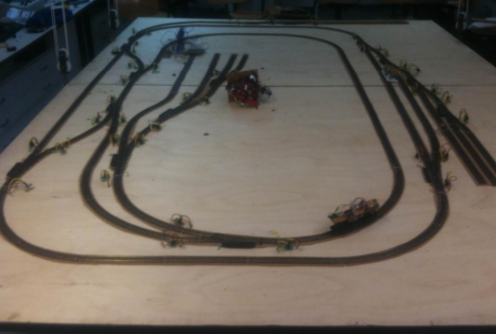
\includegraphics[width=0.5\textwidth]{imagens/maquete}
\caption{Modelo ferroviário desenvolvido no laboratório GRACO-UnB \cite{tgivan}}
\label{im::maquete}
\end{figure}  

O modelo foi realizado em 2013 e encontra-se em desuso, pois a forma de comunicação entre o sistema e o computador não faz uso de uma rede muito eficaz.

\section{Definição do problema}

O modelo original \cite{tgtiago} dispunha de 40 I/O's, ou seja, para as entradas e saídas em uma CLP eram necessárias 40 portas digitais. A necessidade de uma grande quantia de cabos para se conectar as entradas do sistema ao módulo I/O do laboratório tornava inviável a manutenção e organização do modelo. O modelo também não podia ser expandido para sistemas de maior complexidade e simular contextos mais realísticos sem aumentar, consequentemente, a quantia de cabos.

O segundo projeto \cite{tgivan} estabeleu uma solução utilizando um circuito multiplexador de 8 bits. A necessidade de menos portas de entradas e saídas tornou o modelo ferroviário mais viável, porém, a programação exigia uma lógica complexa de decodificação dos 8 bits em linguagem {\it ladder} ou  {\it Sequential Function Chart}.

A utilização de um protocolo de rede industrial se tornou necessária, pois possibilitará a redução de fios sem aumentar a complexidade da programação da CLP.

\section{Objetivos do projeto}

Este projeto visa tornar uma placa Raspberry Pi em um dispositivo de entrada e saída através de um protocolo industrial de rede de campo para realizar a interface entre o modelo de um sistema ferroviário com o controlador. Desta forma, será possível realizar a diminuição de fios sem aumento de complexidade da programação da CLP.

\section{Apresentação do manuscrito}

